\documentclass[a4paper, 12pt]{article}
%%%%%%%%%%%%%%%%%%%%%%%%%%%%%%%%%%%%%%%%%%%%%%%%%%%%%%%%%%%%%%%%%%%%%%%%%%%%%%%
%                                Basic Packages                               %
%%%%%%%%%%%%%%%%%%%%%%%%%%%%%%%%%%%%%%%%%%%%%%%%%%%%%%%%%%%%%%%%%%%%%%%%%%%%%%%

% Gives us multiple colors.
\usepackage[usenames,dvipsnames,pdftex]{xcolor}
% Lets us style link colors.
\usepackage{hyperref}
% Lets us import images and graphics.
\usepackage{graphicx}
% Lets us use figures in floating environments.
\usepackage{float}
% Lets us create multiple columns.
\usepackage{multicol}
% Gives us better math syntax.
\usepackage{amsmath,amsfonts,mathtools,amsthm,amssymb}
% Lets us strikethrough text.
\usepackage{cancel}
% Lets us edit the caption of a figure.
\usepackage{caption}
% Lets us import pdf directly in our tex code.
\usepackage{pdfpages}
% Lets us do algorithm stuff.
\usepackage[ruled,vlined,linesnumbered]{algorithm2e}
% Use a smiley face for our qed symbol.
\usepackage{tikzsymbols}
% \usepackage{fullpage} %%smaller margins
\usepackage[shortlabels]{enumitem}

\setlist[enumerate]{font={\bfseries}} % global settings, for all lists

\usepackage{setspace}
\usepackage[margin=1in, headsep=12pt]{geometry}
\usepackage{wrapfig}
\usepackage{listings}
\usepackage{parskip}

\definecolor{codegreen}{rgb}{0,0.6,0}
\definecolor{codegray}{rgb}{0.5,0.5,0.5}
\definecolor{codepurple}{rgb}{0.58,0,0.82}
\definecolor{backcolour}{rgb}{0.95,0.95,0.95}

\lstdefinestyle{mystyle}{
    backgroundcolor=\color{backcolour},   
    commentstyle=\color{codegreen},
    keywordstyle=\color{magenta},
    numberstyle=\tiny\color{codegray},
    stringstyle=\color{codepurple},
    basicstyle=\ttfamily\footnotesize,
    breakatwhitespace=false,         
    breaklines=true,                 
    captionpos=b,                    
    keepspaces=true,                 
    numbers=left,                    
    numbersep=5pt,                  
    showspaces=false,                
    showstringspaces=false,
    showtabs=false,                  
    tabsize=2,
    numbers=none
}

\lstset{style=mystyle}
\def\class{article}


%%%%%%%%%%%%%%%%%%%%%%%%%%%%%%%%%%%%%%%%%%%%%%%%%%%%%%%%%%%%%%%%%%%%%%%%%%%%%%%
%                                Basic Settings                               %
%%%%%%%%%%%%%%%%%%%%%%%%%%%%%%%%%%%%%%%%%%%%%%%%%%%%%%%%%%%%%%%%%%%%%%%%%%%%%%%

%%%%%%%%%%%%%
%  Symbols  %
%%%%%%%%%%%%%

\let\implies\Rightarrow
\let\impliedby\Leftarrow
\let\iff\Leftrightarrow
\let\epsilon\varepsilon
%%%%%%%%%%%%
%  Tables  %
%%%%%%%%%%%%

\setlength{\tabcolsep}{5pt}
\renewcommand\arraystretch{1.5}

%%%%%%%%%%%%%%
%  SI Unitx  %
%%%%%%%%%%%%%%

\usepackage{siunitx}
\sisetup{locale = FR}

%%%%%%%%%%
%  TikZ  %
%%%%%%%%%%

\usepackage[framemethod=TikZ]{mdframed}
\usepackage{tikz}
\usepackage{tikz-cd}
\usepackage{tikzsymbols}

\usetikzlibrary{intersections, angles, quotes, calc, positioning}
\usetikzlibrary{arrows.meta}

\tikzset{
    force/.style={thick, {Circle[length=2pt]}-stealth, shorten <=-1pt}
}

%%%%%%%%%%%%%%%
%  PGF Plots  %
%%%%%%%%%%%%%%%

\usepackage{pgfplots}
\pgfplotsset{width=10cm, compat=newest}

%%%%%%%%%%%%%%%%%%%%%%%
%  Center Title Page  %
%%%%%%%%%%%%%%%%%%%%%%%

\usepackage{titling}
\renewcommand\maketitlehooka{\null\mbox{}\vfill}
\renewcommand\maketitlehookd{\vfill\null}

%%%%%%%%%%%%%%%%%%%%%%%%%%%%%%%%%%%%%%%%%%%%%%%%%%%%%%%
%  Create a grey background in the middle of the PDF  %
%%%%%%%%%%%%%%%%%%%%%%%%%%%%%%%%%%%%%%%%%%%%%%%%%%%%%%%

\usepackage{eso-pic}
\newcommand\definegraybackground{
    \definecolor{reallylightgray}{HTML}{FAFAFA}
    \AddToShipoutPicture{
        \ifthenelse{\isodd{\thepage}}{
            \AtPageLowerLeft{
                \put(\LenToUnit{\dimexpr\paperwidth-222pt},0){
                    \color{reallylightgray}\rule{222pt}{297mm}
                }
            }
        }
        {
            \AtPageLowerLeft{
                \color{reallylightgray}\rule{222pt}{297mm}
            }
        }
    }
}

%%%%%%%%%%%%%%%%%%%%%%%%
%  Modify Links Color  %
%%%%%%%%%%%%%%%%%%%%%%%%

\hypersetup{
    % Enable highlighting links.
    colorlinks,
    % Change the color of links to blue.
    urlcolor=blue,
    % Change the color of citations to black.
    citecolor={black},
    % Change the color of url's to blue with some black.
    linkcolor={blue!80!black}
}

%%%%%%%%%%%%%%%%%%
% Fix WrapFigure %
%%%%%%%%%%%%%%%%%%

\newcommand{\wrapfill}{\par\ifnum\value{WF@wrappedlines}>0
        \parskip=0pt
        \addtocounter{WF@wrappedlines}{-1}%
        \null\vspace{\arabic{WF@wrappedlines}\baselineskip}%
        \WFclear
    \fi}

%%%%%%%%%%%%%%%%%
% Multi Columns %
%%%%%%%%%%%%%%%%%

\let\multicolmulticols\multicols
\let\endmulticolmulticols\endmulticols

\RenewDocumentEnvironment{multicols}{mO{}}
{%
    \ifnum#1=1
        #2%
    \else % More than 1 column
        \multicolmulticols{#1}[#2]
    \fi
}
{%
    \ifnum#1=1
    \else % More than 1 column
        \endmulticolmulticols
    \fi
}

\newlength{\thickarrayrulewidth}
\setlength{\thickarrayrulewidth}{5\arrayrulewidth}


%%%%%%%%%%%%%%%%%%%%%%%%%%%%%%%%%%%%%%%%%%%%%%%%%%%%%%%%%%%%%%%%%%%%%%%%%%%%%%%
%                           School Specific Commands                          %
%%%%%%%%%%%%%%%%%%%%%%%%%%%%%%%%%%%%%%%%%%%%%%%%%%%%%%%%%%%%%%%%%%%%%%%%%%%%%%%

%%%%%%%%%%%%%%%%%%%%%%%%%%%
%  Initiate New Counters  %
%%%%%%%%%%%%%%%%%%%%%%%%%%%

\newcounter{lecturecounter}

%%%%%%%%%%%%%%%%%%%%%%%%%%
%  Helpful New Commands  %
%%%%%%%%%%%%%%%%%%%%%%%%%%

\makeatletter

\newcommand\resetcounters{
    % Reset the counters for subsection, subsubsection and the definition
    % all the custom environments.
    \setcounter{subsection}{0}
    \setcounter{subsubsection}{0}
    \setcounter{definition0}{0}
    \setcounter{paragraph}{0}
    \setcounter{theorem}{0}
    \setcounter{claim}{0}
    \setcounter{corollary}{0}
    \setcounter{proposition}{0}
    \setcounter{lemma}{0}
    \setcounter{exercise}{0}
    \setcounter{problem}{0}
    
    \setcounter{subparagraph}{0}
    % \@ifclasswith\class{nocolor}{
    %     \setcounter{definition}{0}
    % }{}
}

%%%%%%%%%%%%%%%%%%%%%
%  Lecture Command  %
%%%%%%%%%%%%%%%%%%%%%

\usepackage{xifthen}

% EXAMPLE:
% 1. \lecture{Oct 17 2022 Mon (08:46:48)}{Lecture Title}
% 2. \lecture[4]{Oct 17 2022 Mon (08:46:48)}{Lecture Title}
% 3. \lecture{Oct 17 2022 Mon (08:46:48)}{}
% 4. \lecture[4]{Oct 17 2022 Mon (08:46:48)}{}
% Parameters:
% 1. (Optional) lecture number.
% 2. Time and date of lecture.
% 3. Lecture Title.
\def\@lecture{}
\def\@lectitle{}
\def\@leccount{}
\newcommand\lecture[3]{
    \newpage

    % Check if user passed the lecture title or not.
    \def\@leccount{Lecture #1}
    \ifthenelse{\isempty{#3}}{
        \def\@lecture{Lecture #1}
        \def\@lectitle{Lecture #1}
    }{
        \def\@lecture{Lecture #1: #3}
        \def\@lectitle{#3}
    }

    \setcounter{section}{#1}
    \renewcommand\thesubsection{#1.\arabic{subsection}}
    
    \phantomsection
    \addcontentsline{toc}{section}{\@lecture}
    \resetcounters

    \begin{mdframed}
        \begin{center}
            \Large \textbf{\@leccount}
            
            \vspace*{0.2cm}
            
            \large \@lectitle
            
            
            \vspace*{0.2cm}

            \normalsize #2
        \end{center}
    \end{mdframed}

}

%%%%%%%%%%%%%%%%%%%%
%  Import Figures  %
%%%%%%%%%%%%%%%%%%%%

\usepackage{import}
\pdfminorversion=7

% EXAMPLE:
% 1. \incfig{limit-graph}
% 2. \incfig[0.4]{limit-graph}
% Parameters:
% 1. The figure name. It should be located in figures/NAME.tex_pdf.
% 2. (Optional) The width of the figure. Example: 0.5, 0.35.
\newcommand\incfig[2][1]{%
    \def\svgwidth{#1\columnwidth}
    \import{./figures/}{#2.pdf_tex}
}

\begingroup\expandafter\expandafter\expandafter\endgroup
\expandafter\ifx\csname pdfsuppresswarningpagegroup\endcsname\relax
\else
    \pdfsuppresswarningpagegroup=1\relax
\fi

%%%%%%%%%%%%%%%%%
% Fancy Headers %
%%%%%%%%%%%%%%%%%

\usepackage{fancyhdr}

% Force a new page.
\newcommand\forcenewpage{\clearpage\mbox{~}\clearpage\newpage}

% This command makes it easier to manage my headers and footers.
\newcommand\createintro{
    % Use roman page numbers (e.g. i, v, vi, x, ...)
    \pagenumbering{roman}

    % Display the page style.
    \maketitle
    % Make the title pagestyle empty, meaning no fancy headers and footers.
    \thispagestyle{empty}
    % Create a newpage.
    \newpage

    % Input the intro.tex page if it exists.
    \IfFileExists{intro.tex}{ % If the intro.tex file exists.
        % Input the intro.tex file.
        \textbf{Course}: MATH 16300: Honors Calculus III

\textbf{Section}: 43

\textbf{Professor}: Minjae Park

\textbf{At}: The University of Chicago

\textbf{Quarter}: Spring 2023

\textbf{Course materials}: Calculus by Spivak (4th Edition), Calculus On Manifolds by Spivak

\vspace{1cm}
\textbf{Disclaimer}: This document will inevitably contain some mistakes, both simple typos and serious logical and mathematical errors. Take what you read with a grain of salt as it is made by an undergraduate student going through the learning process himself. If you do find any error, I would really appreciate it if you can let me know by email at \href{mailto:conghungletran@gmail.com}{conghungletran@gmail.com}.

        % Make the pagestyle fancy for the intro.tex page.
        \pagestyle{fancy}

        % Remove the line for the header.
        \renewcommand\headrulewidth{0pt}

        % Remove all header stuff.
        \fancyhead{}

        % Add stuff for the footer in the center.
        % \fancyfoot[C]{
        %   \textit{For more notes like this, visit
        %   \href{\linktootherpages}{\shortlinkname}}. \\
        %   \vspace{0.1cm}
        %   \hrule
        %   \vspace{0.1cm}
        %   \@author, \\
        %   \term: \academicyear, \\
        %   Last Update: \@date, \\
        %   \faculty
        % }

        \newpage
    }{ % If the intro.tex file doesn't exist.
        % Force a \newpageage.
        % \forcenewpage
        \newpage
    }

    % Remove the center stuff we did above, and replace it with just the page
    % number, which is still in roman numerals.
    \fancyfoot[C]{\thepage}
    % Add the table of contents.
    \tableofcontents
    % Force a new page.
    \newpage

    % Move the page numberings back to arabic, from roman numerals.
    \pagenumbering{arabic}
    % Set the page number to 1.
    \setcounter{page}{1}

    % Add the header line back.
    \renewcommand\headrulewidth{0.4pt}
    % In the top right, add the lecture title.
    \fancyhead[R]{\footnotesize \@lecture}
    % In the top left, add the author name.
    \fancyhead[L]{\footnotesize \@author}
    % In the bottom center, add the page.
    \fancyfoot[C]{\thepage}
    % Add a nice gray background in the middle of all the upcoming pages.
    % \definegraybackground
}

\makeatother


%%%%%%%%%%%%%%%%%%%%%%%%%%%%%%%%%%%%%%%%%%%%%%%%%%%%%%%%%%%%%%%%%%%%%%%%%%%%%%%
%                               Custom Commands                               %
%%%%%%%%%%%%%%%%%%%%%%%%%%%%%%%%%%%%%%%%%%%%%%%%%%%%%%%%%%%%%%%%%%%%%%%%%%%%%%%

%%%%%%%%%%%%
%  Circle  %
%%%%%%%%%%%%

\newcommand*\circled[1]{\tikz[baseline= (char.base)]{
        \node[shape=circle,draw,inner sep=1pt] (char) {#1};}
}

%%%%%%%%%%%%%%%%%%%
%  Todo Commands  %
%%%%%%%%%%%%%%%%%%%

% \usepackage{xargs}
% \usepackage[colorinlistoftodos]{todonotes}

% \makeatletter

% \@ifclasswith\class{working}{
%     \newcommandx\unsure[2][1=]{\todo[linecolor=red,backgroundcolor=red!25,bordercolor=red,#1]{#2}}
%     \newcommandx\change[2][1=]{\todo[linecolor=blue,backgroundcolor=blue!25,bordercolor=blue,#1]{#2}}
%     \newcommandx\info[2][1=]{\todo[linecolor=OliveGreen,backgroundcolor=OliveGreen!25,bordercolor=OliveGreen,#1]{#2}}
%     \newcommandx\improvement[2][1=]{\todo[linecolor=Plum,backgroundcolor=Plum!25,bordercolor=Plum,#1]{#2}}

%     \newcommand\listnotes{
%         \newpage
%         \listoftodos[Notes]
%     }
% }{
%     \newcommandx\unsure[2][1=]{}
%     \newcommandx\change[2][1=]{}
%     \newcommandx\info[2][1=]{}
%     \newcommandx\improvement[2][1=]{}

%     \newcommand\listnotes{}
% }

% \makeatother

%%%%%%%%%%%%%
%  Correct  %
%%%%%%%%%%%%%

% EXAMPLE:
% 1. \correct{INCORRECT}{CORRECT}
% Parameters:
% 1. The incorrect statement.
% 2. The correct statement.
\definecolor{correct}{HTML}{009900}
\newcommand\correct[2]{{\color{red}{#1 }}\ensuremath{\to}{\color{correct}{ #2}}}


%%%%%%%%%%%%%%%%%%%%%%%%%%%%%%%%%%%%%%%%%%%%%%%%%%%%%%%%%%%%%%%%%%%%%%%%%%%%%%%
%                                 Environments                                %
%%%%%%%%%%%%%%%%%%%%%%%%%%%%%%%%%%%%%%%%%%%%%%%%%%%%%%%%%%%%%%%%%%%%%%%%%%%%%%%

\usepackage{varwidth}
\usepackage{thmtools}
\usepackage[most,many,breakable]{tcolorbox}

\tcbuselibrary{theorems,skins,hooks}
\usetikzlibrary{arrows,calc,shadows.blur}

%%%%%%%%%%%%%%%%%%%
%  Define Colors  %
%%%%%%%%%%%%%%%%%%%

% color prototype
% \definecolor{color}{RGB}{45, 111, 177}

% ESSENTIALS: 
\definecolor{myred}{HTML}{c74540}
\definecolor{myblue}{HTML}{072b85}
\definecolor{mygreen}{HTML}{388c46}
\definecolor{myblack}{HTML}{000000}

\colorlet{definition_color}{myred}

\colorlet{theorem_color}{myblue}
\colorlet{lemma_color}{myblue}
\colorlet{prop_color}{myblue}
\colorlet{corollary_color}{myblue}
\colorlet{claim_color}{myblue}

\colorlet{proof_color}{myblack}
\colorlet{example_color}{myblack}
\colorlet{exercise_color}{myblack}

% MISCS: 
%%%%%%%%%%%%%%%%%%%%%%%%%%%%%%%%%%%%%%%%%%%%%%%%%%%%%%%%%
%  Create Environments Styles Based on Given Parameter  %
%%%%%%%%%%%%%%%%%%%%%%%%%%%%%%%%%%%%%%%%%%%%%%%%%%%%%%%%%

% \mdfsetup{skipabove=1em,skipbelow=0em}

%%%%%%%%%%%%%%%%%%%%%%
%  Helpful Commands  %
%%%%%%%%%%%%%%%%%%%%%%

% EXAMPLE:
% 1. \createnewtheoremstyle{thmdefinitionbox}{}{}
% 2. \createnewtheoremstyle{thmtheorembox}{}{}
% 3. \createnewtheoremstyle{thmproofbox}{qed=\qedsymbol}{
%       rightline=false, topline=false, bottomline=false
%    }
% Parameters:
% 1. Theorem name.
% 2. Any extra parameters to pass directly to declaretheoremstyle.
% 3. Any extra parameters to pass directly to mdframed.
\newcommand\createnewtheoremstyle[3]{
    \declaretheoremstyle[
        headfont=\bfseries\sffamily, bodyfont=\normalfont, #2,
        mdframed={
                #3,
            },
    ]{#1}
}

% EXAMPLE:
% 1. \createnewcoloredtheoremstyle{thmdefinitionbox}{definition}{}{}
% 2. \createnewcoloredtheoremstyle{thmexamplebox}{example}{}{
%       rightline=true, leftline=true, topline=true, bottomline=true
%     }
% 3. \createnewcoloredtheoremstyle{thmproofbox}{proof}{qed=\qedsymbol}{backgroundcolor=white}
% Parameters:
% 1. Theorem name.
% 2. Color of theorem.
% 3. Any extra parameters to pass directly to declaretheoremstyle.
% 4. Any extra parameters to pass directly to mdframed.

% change backgroundcolor to #2!5 if user wants a colored backdrop to theorem environments. It's a cool color theme, but there's too much going on in the page.
\newcommand\createnewcoloredtheoremstyle[4]{
    \declaretheoremstyle[
        headfont=\bfseries\sffamily\color{#2},
        bodyfont=\normalfont,
        headpunct=,
        headformat = \NAME~\NUMBER\NOTE \hfill\smallskip\linebreak,
        #3,
        mdframed={
                outerlinewidth=0.75pt,
                rightline=false,
                leftline=false,
                topline=false,
                bottomline=false,
                backgroundcolor=white,
                skipabove = 5pt,
                skipbelow = 0pt,
                linecolor=#2,
                innertopmargin = 0pt,
                innerbottommargin = 0pt,
                innerrightmargin = 4pt,
                innerleftmargin= 6pt,
                leftmargin = -6pt,
                #4,
            },
    ]{#1}
}



%%%%%%%%%%%%%%%%%%%%%%%%%%%%%%%%%%%
%  Create the Environment Styles  %
%%%%%%%%%%%%%%%%%%%%%%%%%%%%%%%%%%%

\makeatletter
\@ifclasswith\class{nocolor}{
    % Environments without color.

    % ESSENTIALS:
    \createnewtheoremstyle{thmdefinitionbox}{}{}
    \createnewtheoremstyle{thmtheorembox}{}{}
    \createnewtheoremstyle{thmproofbox}{qed=\qedsymbol}{}
    \createnewtheoremstyle{thmcorollarybox}{}{}
    \createnewtheoremstyle{thmlemmabox}{}{}
    \createnewtheoremstyle{thmclaimbox}{}{}
    \createnewtheoremstyle{thmexamplebox}{}{}

    % MISCS: 
    \createnewtheoremstyle{thmpropbox}{}{}
    \createnewtheoremstyle{thmexercisebox}{}{}
    \createnewtheoremstyle{thmexplanationbox}{}{}
    \createnewtheoremstyle{thmremarkbox}{}{}
    
    % STYLIZED MORE BELOW
    \createnewtheoremstyle{thmquestionbox}{}{}
    \createnewtheoremstyle{thmsolutionbox}{qed=\qedsymbol}{}
}{
    % Environments with color.

    % ESSENTIALS: definition, theorem, proof, corollary, lemma, claim, example
    \createnewcoloredtheoremstyle{thmdefinitionbox}{definition_color}{}{leftline=false}
    \createnewcoloredtheoremstyle{thmtheorembox}{theorem_color}{}{leftline=false}
    \createnewcoloredtheoremstyle{thmproofbox}{proof_color}{qed=\qedsymbol}{}
    \createnewcoloredtheoremstyle{thmcorollarybox}{corollary_color}{}{leftline=false}
    \createnewcoloredtheoremstyle{thmlemmabox}{lemma_color}{}{leftline=false}
    \createnewcoloredtheoremstyle{thmpropbox}{prop_color}{}{leftline=false}
    \createnewcoloredtheoremstyle{thmclaimbox}{claim_color}{}{leftline=false}
    \createnewcoloredtheoremstyle{thmexamplebox}{example_color}{}{}
    \createnewcoloredtheoremstyle{thmexplanationbox}{example_color}{qed=\qedsymbol}{}
    \createnewcoloredtheoremstyle{thmremarkbox}{theorem_color}{}{}

    \createnewcoloredtheoremstyle{thmmiscbox}{black}{}{}

    \createnewcoloredtheoremstyle{thmexercisebox}{exercise_color}{}{}
    \createnewcoloredtheoremstyle{thmproblembox}{theorem_color}{}{leftline=false}
    \createnewcoloredtheoremstyle{thmsolutionbox}{mygreen}{qed=\qedsymbol}{}
}
\makeatother

%%%%%%%%%%%%%%%%%%%%%%%%%%%%%
%  Create the Environments  %
%%%%%%%%%%%%%%%%%%%%%%%%%%%%%
\declaretheorem[numberwithin=section, style=thmdefinitionbox,     name=Definition]{definition}
\declaretheorem[numberwithin=section, style=thmtheorembox,     name=Theorem]{theorem}
\declaretheorem[numbered=no,          style=thmexamplebox,     name=Example]{example}
\declaretheorem[numberwithin=section, style=thmtheorembox,       name=Claim]{claim}
\declaretheorem[numberwithin=section, style=thmcorollarybox,   name=Corollary]{corollary}
\declaretheorem[numberwithin=section, style=thmpropbox,        name=Proposition]{proposition}
\declaretheorem[numberwithin=section, style=thmlemmabox,       name=Lemma]{lemma}
\declaretheorem[numberwithin=section, style=thmexercisebox,    name=Exercise]{exercise}
\declaretheorem[numbered=no,          style=thmproofbox,       name=Proof]{proof0}
\declaretheorem[numbered=no,          style=thmexplanationbox, name=Explanation]{explanation}
\declaretheorem[numbered=no,          style=thmsolutionbox,    name=Solution]{solution}
\declaretheorem[numberwithin=section,          style=thmproblembox,     name=Problem]{problem}
\declaretheorem[numbered=no,          style=thmmiscbox,    name=Intuition]{intuition}
\declaretheorem[numbered=no,          style=thmmiscbox,    name=Goal]{goal}
\declaretheorem[numbered=no,          style=thmmiscbox,    name=Recall]{recall}
\declaretheorem[numbered=no,          style=thmmiscbox,    name=Motivation]{motivation}
\declaretheorem[numbered=no,          style=thmmiscbox,    name=Remark]{remark}
\declaretheorem[numbered=no,          style=thmmiscbox,    name=Observe]{observe}
\declaretheorem[numbered=no,          style=thmmiscbox,    name=Question]{question}


%%%%%%%%%%%%%%%%%%%%%%%%%%%%
%  Edit Proof Environment  %
%%%%%%%%%%%%%%%%%%%%%%%%%%%%

\renewenvironment{proof}[2][\proofname]{
    % \vspace{-12pt}
    \begin{proof0} [#2]
        }{\end{proof0}}

\theoremstyle{definition}

\newtheorem*{notation}{Notation}
\newtheorem*{previouslyseen}{As previously seen}
\newtheorem*{property}{Property}
% \newtheorem*{intuition}{Intuition}
% \newtheorem*{goal}{Goal}
% \newtheorem*{recall}{Recall}
% \newtheorem*{motivation}{Motivation}
% \newtheorem*{remark}{Remark}
% \newtheorem*{observe}{Observe}

\author{Hung C. Le Tran}


%%%% MATH SHORTHANDS %%%%
%% blackboard bold math capitals
\DeclareMathOperator*{\esssup}{ess\,sup}
\DeclareMathOperator*{\Hom}{Hom}
\newcommand{\bbf}{\mathbb{F}}
\newcommand{\bbn}{\mathbb{N}}
\newcommand{\bbq}{\mathbb{Q}}
\newcommand{\bbr}{\mathbb{R}}
\newcommand{\bbz}{\mathbb{Z}}
\newcommand{\bbc}{\mathbb{C}}
\newcommand{\bbk}{\mathbb{K}}
\newcommand{\bbm}{\mathbb{M}}
\newcommand{\bbp}{\mathbb{P}}
\newcommand{\bbe}{\mathbb{E}}

\newcommand{\bfw}{\mathbf{w}}
\newcommand{\bfx}{\mathbf{x}}
\newcommand{\bfX}{\mathbf{X}}
\newcommand{\bfy}{\mathbf{y}}
\newcommand{\bfyhat}{\mathbf{\hat{y}}}

\newcommand{\calb}{\mathcal{B}}
\newcommand{\calf}{\mathcal{F}}
\newcommand{\calt}{\mathcal{T}}
\newcommand{\call}{\mathcal{L}}
\renewcommand{\phi}{\varphi}

% Universal Math Shortcuts
\newcommand{\st}{\hspace*{2pt}\text{s.t.}\hspace*{2pt}}
\newcommand{\pffwd}{\hspace*{2pt}\fbox{\(\Rightarrow\)}\hspace*{10pt}}
\newcommand{\pfbwd}{\hspace*{2pt}\fbox{\(\Leftarrow\)}\hspace*{10pt}}
\newcommand{\contra}{\ensuremath{\Rightarrow\Leftarrow}}
\newcommand{\cvgn}{\xrightarrow{n \to \infty}}
\newcommand{\cvgj}{\xrightarrow{j \to \infty}}

\newcommand{\im}{\mathrm{im}}
\newcommand{\innerproduct}[2]{\langle #1, #2 \rangle}
\newcommand*{\conj}[1]{\overline{#1}}

% https://tex.stackexchange.com/questions/438612/space-between-exists-and-forall
% https://tex.stackexchange.com/questions/22798/nice-looking-empty-set
\let\oldforall\forall
\renewcommand{\forall}{\;\oldforall\; }
\let\oldexist\exists
\renewcommand{\exists}{\;\oldexist\; }
\newcommand\existu{\;\oldexist!\: }
\let\oldemptyset\emptyset
\let\emptyset\varnothing


\renewcommand{\_}[1]{\underline{#1}}
\DeclarePairedDelimiter{\abs}{\lvert}{\rvert}
\DeclarePairedDelimiter{\norm}{\lVert}{\rVert}
\DeclarePairedDelimiter\ceil{\lceil}{\rceil}
\DeclarePairedDelimiter\floor{\lfloor}{\rfloor}
\setlength\parindent{0pt}
\setlength{\headheight}{12.0pt}
\addtolength{\topmargin}{-12.0pt}


% Default skipping, change if you want more spacing
% \thinmuskip=3mu
% \medmuskip=4mu plus 2mu minus 4mu
% \thickmuskip=5mu plus 5mu

% \DeclareMathOperator{\ext}{ext}
% \DeclareMathOperator{\bridge}{bridge}
\title{CMSC 25300: Mathematical Foundations of ML \\ \large Problem Set 6}
\date{17 Nov 2023}
\author{Hung Le Tran}
\begin{document}
\maketitle
\setcounter{section}{6}
\begin{problem} [Problem 1]
\end{problem}
\begin{solution}
    \textbf{(a)}
    Let \[
    f(w) = \norm{\Phi w - y}^2 + \lambda \norm{w}^2 
    \]
    then \begin{align*}
        f(w) &= w^T \Phi^T \Phi w - 2 w^T \Phi^T y + y^T y + \lambda w^T w\\
        \implies \nabla_w f(w) &= 2\Phi^T \Phi w - 2\Phi^T y + 2\lambda w
    \end{align*}
    is zero when \begin{align*}
        2\Phi^T \Phi w - 2\Phi^T y + 2\lambda w_{krr} & = 0 \\
        \implies w_{krr} &= (\Phi^T \Phi + \lambda I)^{-1}\Phi^T y \\
        &= \Phi^T (\Phi^T \Phi + \lambda I)^{-1} y
    \end{align*}
    via SVD of $\Phi$, as similar to regular ridge regression.

    \textbf{(b)(i)}    We want to write $w_{krr} = \Phi^T \alpha$.  From (a), \begin{align}
        \alpha &= (\Phi^T \Phi + \lambda I)^{-1} y \\
        &= (K + \lambda I)^{-1}y
    \end{align}

    \textbf{(b)(ii)} To make prediction on new sample $z$: 
    \begin{align*}
        \bfyhat &= w^T_{krr}\Phi(z) \\
        &= (\Phi^T \alpha)^T \Phi(z) \\
        &= \alpha^T (\Phi \Phi(z)) \\
        &= \alpha^T k(\bfX, z) \\
    \end{align*}

    \textbf{(c)} Mathematically, \[
    k(x_i, x_j) = \phi(x_i)^T \phi(x_j)
    \]
    and \[
    K = \Phi \Phi^T
    \]
    We have $\Phi$ to increase the dimensionality of the feature space, so that linear LS on the new feature space can create better-fit decision boundaries that are not achievable in lower dimensions. However, this comes with the cost of more data storage, which $k$ and $K$ solves, by directly computing $\Phi(x_i)^T \Phi(x_j)$, in order to construct $K = \Phi\Phi^T$, which is what we really need to calculate $w_{krr}$.

    \textbf{(d)} I chose $d$ because the simulated data suggests a circular decision boundary, which can be generated by \[
    (x_1^2 + x_2^2)^2 - r^2 = 0
    \]
    for some $r$, which is a degree-2 polynomial.

\begin{lstlisting} [language=python]
import numpy as np
import matplotlib.pyplot as plt
import numpy.linalg as la

np.random.seed(10)

n = 200
p = 2
X = 2 * (np.random.rand(n, p) - .5)
radius = 0.5
distances = np.linalg.norm(X, axis = 1)

y = np.where(distances < radius, 1, -1)

plt.figure(1)
plt.scatter(X[:, 0], X[:, 1], 50, c = y)
plt.colorbar()
plt.xlabel('feature 1')
plt.ylabel('feature 2')
plt.title('2d training samples colored by label')
plt.show()

c = 1
lam = 1
d = 2
innerProds = X @ X.T

### YOUR CODE STARTS HERE ###
K = np.power(innerProds + c, d)
alpha = la.inv((K + lam * np.identity(n))) @ y
yhat = K @ alpha
### YOUR CODE ENDS HERE ###

y2 = np.array(np.sign(yhat))
plt.figure(2)
plt.scatter(X[:, 0], X[:, 1], 50, c=y2)
plt.colorbar()
plt.xlabel('feature 1')
plt.ylabel('feature 2')
plt.title('2d training samples colored by predicted label')
plt.show()

ntest = 2000
Xtest = 2*(np.random.rand(ntest, p) - .5)

# make predictions on test data
innerProds_test = Xtest@X.T
### YOUR CODE STARTS HERE
K_test = np.power(innerProds_test + c, d)
ytest = K_test @ alpha
### YOUR CODE ENDS HERE

plt.figure(3)
plt.scatter(Xtest[:, 0], Xtest[:, 1], 50, c = np.array(ytest))
plt.colorbar()
plt.xlabel('feature 1') 
plt.ylabel('feature 2')
plt.title('2d test samples colored by PREDICTED label (before taking sign)')
plt.show()
\end{lstlisting}
which plots
\begin{center}
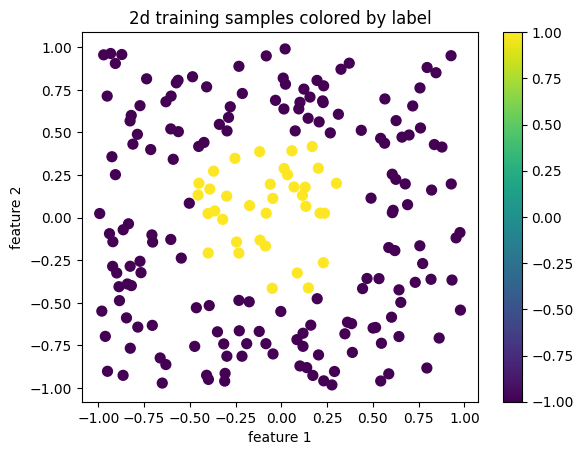
\includegraphics[width=9cm]{./figures/6.1d.1.png}
\end{center}
\begin{center}
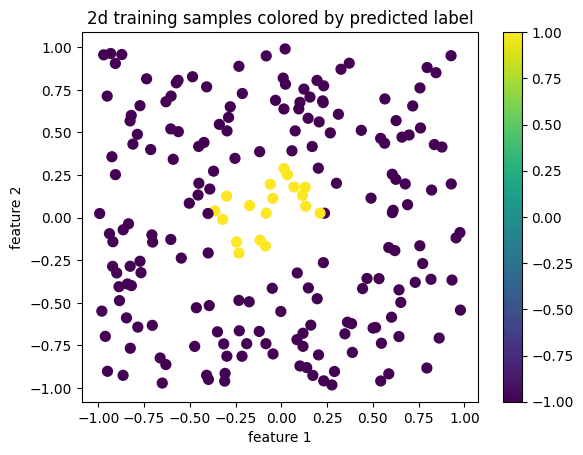
\includegraphics[width=9cm]{./figures/6.1d.2.png}
\end{center}
\begin{center}
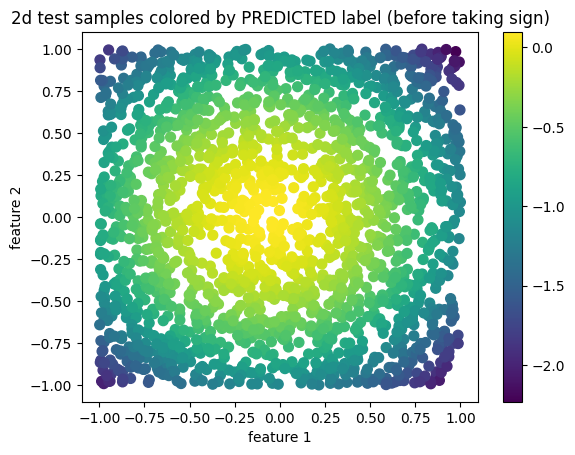
\includegraphics[width=9cm]{./figures/6.1d.3.png}
\end{center}
\end{solution}

\begin{problem} [Problem 2]
\end{problem}
\begin{solution}
\textbf{(a)(i)}
If $g_1, g_2$ are convex then
\begin{align*}
g(w) - g(v) &= (g_1(w) - g_1(v)) + (g_2(w) - g_2(v)) \\
&\geq \nabla g_1(v)^T (w-v) + \nabla g_2(v)^T (w-v) \\
&= \nabla g^T (w - v)
\end{align*}
which implies $g$ is also convex.

\textbf{(a)(ii)}
\begin{align*}
    g(w) &= g(v) + \nabla g(v)^T  (w-v) + \frac{1}{2}(w-v)^T \nabla^2_g (w-v) \\
    &= v^tKv + 2(Kv)^T(w-v) + (w-v)^TK(w-v) 
\end{align*}
has $g(v) + \nabla g(v)^T = v^TKv + 2(Kv)^T(w-v)$ as the first-order approximation. The second-order term, $(w-v)^TK(w-v) \geq 0$ since $K$ is positive semidefinite. Therefore \[
g(w)  \geq g(v) + \nabla g(v)^T (w-v)
\]
\textbf{(b)} If after $t$ steps, all points are correctly classified, then no loss is incurred on the samples. Therefore $f(\alpha^{(t)}) = \lambda \alpha^{(t)^T} K \alpha^{(t)}$ with only the regularization term. 

Consequently, $\alpha^{(t+1)} = \alpha^{(t)} - 2 \tau \lambda K \alpha^{(t)}$, since there is no contribution from the gradient of loss function term.

\textbf{(c)} If we keep iterating GD, we might no longer correctly classify for all traning samples and there would be loss incurred due to error on the training samples. Therefore it might not remain true that the error term on training samples is zero on later iterations of GD.

At the optimal value $\alpha^*$, 
\begin{align*}
    0 &= \nabla_\alpha f|_{\alpha = \alpha^*}\\
    &= \sum_{i=1}^{n} \1_{\{y_i k_i^T \alpha^* < 1\}} (-y_i k_i) + 2 \lambda K \alpha^*\\
    \implies \sum_{i=1}^{n} \1_{\{y_i k_i^T \alpha^* < 1\}} (y_i k_i) &= 2 \lambda K \alpha^*
\end{align*}
What this tells us is that at the optimal solution, since $RHS \neq 0$, $LHS \neq 0$ too. It follows that it must classify at least 1 training sample wrongly.
\end{solution}

\begin{problem} [Problem 3]
\end{problem}
\begin{solution}
\textbf{(a)}
\begin{lstlisting} [language=python]
import numpy as np
def matrix_completion_svt (
mat_shape : tuple ,
obs_vals : np.ndarray ,
obs_idcs : tuple ,
trunc_rank : int ,
iter_count : int = 100 ,
verbose : bool = False ) -> np . ndarray :
    """ Matrix completion with Singular Value Thresholding
    Parameters :
        mat_shape ( tuple ) : shape of the target matrix
        obs_vals ( np . ndarray ) : a flattened array containing the
        observed values
        obs_idcs ( tuple of np . ndarrays ) : describes the indices of
        the observed values in question
        Given as a tuple with an array of indices for each
        spatial dimension
        Usage : mat [ obs_idcs ] returns a view of the entries in
        question ( can also be used to set values )
        trunc_rank ( int ) : number of singular values to keep .
        Truncates singular values to set matrix to this rank
        iter_count ( int ) : number of iterations to run singular
        value thresholding
        verbose ( bool ) : flag for whether to output the step
        sizes at a given iteration
        
        Output :
        mat_rec ( np . ndarray ) : the recovered matrix
    """
    mat_rec = np.zeros ( mat_shape )
    # TODO 1: set observed entries of mat_rec to obs_vals
    mat_rec[obs_idcs] = obs_vals
    for it in range (1 , 1 + iter_count ) :
        # Apply rank reduction with SVD
        # TODO 2: truncate singular values of mat_rec , save to
        U, S, Vt = np.linalg.svd(mat_rec)
        S_trunc= np.zeros(S.shape)
        S_trunc[:trunc_rank] = S[:trunc_rank]
        mat_rec_new = U @ np.diag(S_trunc) @ Vt
        # Correct for measurements
        # TODO 3: set observed entries of mat_rec_new to obs_vals
        mat_rec_new[obs_idcs] = obs_vals
        # Basic logging
        if verbose and ( it %20==0 or it == iter_count ) :
            rel_update_size = np.linalg.norm(mat_rec_new - mat_rec)/np.linalg.norm(mat_rec)
            print (f" Iteration {it:3d}: relative update size ={rel_update_size:.3e}")
        mat_rec = mat_rec_new
    return mat_rec
# To load the appropriate values from data (for testing purposes) :
sensor_data_file = np.load("sensor_data.npz")
dim = sensor_data_file ["dim"]
sensor_count = sensor_data_file ["sensor_count"]
coords_ref = sensor_data_file ["coords_ref"]
dist_mat_ref = sensor_data_file ["dist_mat_ref"]
obs_dists = sensor_data_file ["obs_dists"]
obs_idcs = tuple ([*sensor_data_file ["obs_idcs"]])

D = matrix_completion_svt(dist_mat_ref.shape, obs_dists, obs_idcs, 3 + 2, 200, True)
\end{lstlisting}
which prints
\begin{lstlisting}
Iteration  20: relative update size =1.293e-02
Iteration  40: relative update size =3.457e-03
Iteration  60: relative update size =2.576e-03
Iteration  80: relative update size =7.624e-04
Iteration 100: relative update size =2.582e-04
Iteration 120: relative update size =1.058e-04
Iteration 140: relative update size =4.588e-05
Iteration 160: relative update size =2.036e-05
Iteration 180: relative update size =9.171e-06
Iteration 200: relative update size =4.178e-06
\end{lstlisting}
\textbf{(b)} $M$ has rank $d$, which means that $\Sigma$ only has its first $d$ entries as non-zero entries. Therefore one can construct $S$ of shape $n \times d$, with zero entries except for its diagonal entries as $\sqrt{\sigma_1}, \sqrt{\sigma_2}, \ldots, \sqrt{\sigma_d}$
which would then give \[
\Sigma = SS^T
\]
Therefore \begin{align*}
M &= U\Sigma U^T \\
&= US S^T U^T \\
&= (US)(US)^T
\end{align*}
Furthermore, $Y = US$ has rank $d$ since its $d$ columns are scaled version of the columns of $U$, which are linearly independent.

\textbf{(c)}
\end{solution}
\begin{lstlisting} [language=python]
def localize_sensors_from_data (
    sensor_count : int ,
    dim : int ,
    obs_dists : np . ndarray ,
    obs_idcs : tuple ,
    anchor_coords : np . ndarray ,
    svt_iter_count : int = 100 ,
    verbose : bool = False ,
    ) -> ( np . ndarray , np . ndarray ) :
    """ Takes in the incomplete distance measurement data and
    recovers the locations of all sensors
    Note that this procedure requires the true location of several
    sensors considered " anchors "
    Parameters :
        sensor_count ( int ) : number of sensors
        dim ( int ) : dimension of the space ( e . g . , dim =2 or dim =3)
        obs_dists ( np . ndarray ) : a 1 D array containing measured distances
        obs_idcs ( tuple of np . ndarrays ) : describes the indices of the observed values in question. Given as a tuple with an array of indices for each spatial dimension
        anchor_coords ( np . ndarray ) : coordinates of the " anchor " points. For simplicity let these be the positions of the first few sensors .
        svt_iter_count ( int ) : number of iterations for singular value thresholding
        verbose ( bool ) : whether to print logging information
    
    Outputs :
    coords_rec ( np . ndarray ) : the recovered coordinates of all sensors. Takes shape ( sensor_count , dim )
    dist_mat_rec ( np . ndarray ) : the recovered ( squared )
    distance matrix between sensors. Takes shape ( sensor_count , sensor_count )( Value is returned to facilitate debugging )
    """
    anchor_count = anchor_coords.shape[0]
    # TODO 3: run SVT to fill in the distance matrix
    dist_mat = matrix_completion_svt((sensor_count, sensor_count), obs_dists, obs_idcs, dim + 2, svt_iter_count, verbose)
    # Now recover sensor coordinates from the distance matrix
    # (using anchor points to find the right alignment)
    M_mat = build_M_mat(dist_mat)
    # Y matrices represent sensor locations in a shifted coordinate system ( with x_1 at the origin)
    Y_raw = factor_psd(M_mat,col_count = dim)
    Y_anchor_ref = anchor_coords - anchor_coords [0, np.newaxis, :]
    # The recovered Y matrix is only unique up to a global
    # rotation since M =( YR ) ( YR ) ^ T = YRR ^ TY ^ T = YY ^ T for orthogonal R
    # so we need to find the appropriate alignment to match
    # the reference positions for the " anchor " sensors
    alignment = find_alignment (Y_raw [:anchor_count], Y_anchor_ref)
    Y_aligned = (Y_raw @ alignment)
    # Shift the coordinates to recover the original X matrix
    # TODO 4: bring back from the shifted coordinate system used in Y_aligned
    sensor_coords = Y_aligned + anchor_coords [0, np.newaxis, :]
    
    if verbose :
        # Extra outputs to help with debugging
        # Find relative magnitude in dist_mat beyond rank ( dim +2)
        svals = np.linalg.svd (dist_mat, compute_uv = False )
        sv_err = np.linalg.norm (svals [dim +2:]) / np.linalg.norm (
        svals)
        print (f"\nDistance matrix rank error: {sv_err:.3e}")
        # Find the error incurred by factoring M_mat
        factor_err = np . linalg . norm ( Y_raw @ Y_raw . T - M_mat ) / np . linalg . norm ( M_mat )
        print (f"Factorization error: {factor_err:.3e}")
        # Find the quality of the alignment against anchor points
        Y_anchor_rec = Y_raw [: anchor_count ] @ alignment
        align_err = np.linalg.norm(Y_anchor_rec - Y_anchor_ref)/np . linalg . norm ( Y_anchor_ref )
        print (f"Alignment error: {np.linalg.norm(align_err):.3e}")
    return sensor_coords , dist_mat
# Example settings to call the function
# Code to load the data is provided in part ( a )
anchor_count = 4
anchor_coords = coords_ref [: anchor_count ]
coords_rec , dist_mat_rec = localize_sensors_from_data (
sensor_count ,
dim ,
obs_dists ,
obs_idcs ,
anchor_coords ,
svt_iter_count = 250 ,
verbose = True ,
)
dist_mat_err = np . linalg . norm ( dist_mat_rec - dist_mat_ref ) / np .linalg . norm ( dist_mat_rec )
coords_err = np . linalg . norm (( coords_rec - coords_ref ) [
anchor_count :]) / np . linalg . norm ( coords_ref [ anchor_count :])
print ()
print (f"Distance matrix error: {dist_mat_err:.3e}" )
print (f"Sensor coordinate error: {coords_err:.3e}" )
\end{lstlisting}
which prints
\begin{lstlisting}
Iteration  20: relative update size =1.293e-02
Iteration  40: relative update size =3.457e-03
Iteration  60: relative update size =2.576e-03
Iteration  80: relative update size =7.624e-04
Iteration 100: relative update size =2.582e-04
Iteration 120: relative update size =1.058e-04
Iteration 140: relative update size =4.588e-05
Iteration 160: relative update size =2.036e-05
Iteration 180: relative update size =9.171e-06
Iteration 200: relative update size =4.178e-06
Iteration 220: relative update size =1.921e-06
Iteration 240: relative update size =8.900e-07
Iteration 250: relative update size =6.075e-07

Distance matrix rank error: 3.034e-06
Factorization error: 5.730e-06
Alignment error: 4.373e-06

Distance matrix error: 1.578e-05
Sensor coordinate error: 1.928e-05
\end{lstlisting}
\end{document}